This problem is a simplification of  \textit{Convex Hull} problem because here we just need to traverse the points, no need to check if traversing is going clockwise or not. Algorithm is the following for $n$ points:
\begin{itemize}
  \item Find the initial point $p_i$ which has \textit{minimum y}, finding minimum of $n$ points is bound by $O(n)$
  \item Sort the remaining points in ascending order according to polar angle that they made with $p$ where it is bound by $O(n \log n)$ because we only spend $O(1)$ time for each  polar angle calculation, in total, that results in $O(n)$ which is dominated by sorting $n$ points.
  \item Traverse the points in the order and put an edge between the current point $p_c$ and the following point $p_f$. Since we are traversing all points, this is $O(n)$.
  \item At the end, put one more edge between $p_c$ and $p_i$ to close the loop and create a polygon. This operation is just a constant time operation, $O(1)$.
\end{itemize}

In short, we have:

\begin{align*}
  \textit{Total Cost} &= Find p_i + \textit{Calculate polar angles with } p_i + Sort points + \textit{Close loop} \\
                      &= O(n) + O(n) + O(n \log n) + O(1) \leq O(n \log n)
\end{align*}

\begin{figure}[ht]
  \centering
  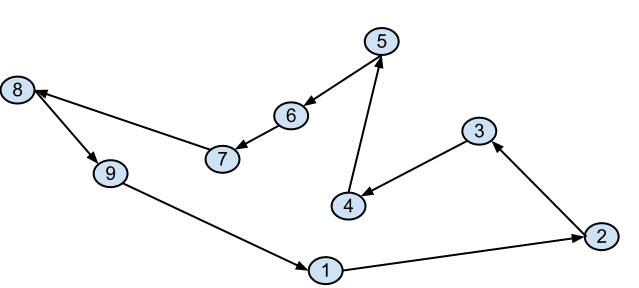
\includegraphics[width=0.75\textwidth]{prob4}
  \caption{Application of our algorithm for 9 points}
  \label{fig:prob4}
\end{figure}